\documentclass[tikz,border=10pt]{standalone}
\usepackage{tikz}
\usepackage{fontawesome5}
\usepackage{amsmath,amssymb}
\usetikzlibrary{arrows.meta,positioning,fit,backgrounds,calc,shadows,shapes.geometric}

% Color definitions
\definecolor{lavenderDark}{RGB}{15, 44, 89}
\definecolor{lavenderDeep}{RGB}{10, 28, 58}
\definecolor{lavenderMedium}{RGB}{29, 78, 158}
\definecolor{lavenderLight}{RGB}{240, 246, 255}
\definecolor{lavenderBorder}{RGB}{180, 205, 237}
\definecolor{prismNavy}{RGB}{15, 44, 89}
\definecolor{prismBlue}{RGB}{29, 78, 158}
\definecolor{prismTeal}{RGB}{13, 148, 136}
\definecolor{prismGold}{RGB}{217, 119, 6}
\definecolor{prismDark}{RGB}{15, 23, 42}
\definecolor{prismSlate}{RGB}{100, 116, 139}
\definecolor{statusFail}{RGB}{220, 38, 38}
\definecolor{cInput}{RGB}{241, 245, 249}
\definecolor{cStem}{RGB}{224, 242, 254}
\definecolor{cStage1}{RGB}{209, 250, 229}
\definecolor{cStage2}{RGB}{254, 243, 199}
\definecolor{cHead}{RGB}{219, 234, 254}

\begin{document}
% Blockchain Block Structure and Cryptographic Chaining Diagram
\begin{tikzpicture}[
  x=1cm, y=1cm,
  blockcard/.style={
    rectangle, rounded corners=6pt, draw=lavenderDark!90, line width=1.1pt,
    fill=white, text width=4.60cm, minimum height=6.20cm,
    inner sep=6pt, drop shadow={shadow xshift=1.2pt, shadow yshift=-1.2pt, opacity=0.15}
  },
  hdrsub/.style={
    rectangle, rounded corners=3pt, draw=prismBlue!70, fill=cStem,
    text width=4.30cm, inner sep=4pt, align=left, font=\fontsize{6.8}{8.0}\selectfont
  },
  txsub/.style={
    rectangle, rounded corners=3pt, draw=prismTeal!70, fill=cStage1,
    text width=4.30cm, inner sep=4pt, align=left, font=\fontsize{6.6}{7.8}\selectfont
  },
  hashsub/.style={
    rectangle, rounded corners=3pt, draw=prismGold!80, fill=cStage2,
    text width=4.30cm, inner sep=4pt, align=left, font=\fontsize{6.8}{8.0}\selectfont
  },
  chainarr/.style={
    -{Stealth[scale=1.1]}, line width=1.6pt, draw=lavenderDark
  }
]

  %============================================================================
  % BLOCK i-1
  %============================================================================
  \node[blockcard] (b_prev) at (-5.4, 0) {};
  \node[anchor=north, font=\fontsize{8.5}{10.5}\selectfont\bfseries, text=prismNavy] at ([yshift=-4pt]b_prev.north) {
    \faCube\ \textbf{BLOCK} $B_{i-1}$ \textit{(Previous)}
  };
  \node[hdrsub, below=0.6cm of b_prev.north] (h_prev) {
    \textbf{Block Header:}\\[1.5pt]
    $\bullet$ Prev Hash: \texttt{0x9f7a...3c21}\\
    $\bullet$ Timestamp: $T_{i-1} = 1730001200$\\
    $\bullet$ Nonce: $n_{i-1} = 48219$\\
    $\bullet$ Merkle Root: \texttt{0x4e8b...1a02}
  };
  \node[txsub, below=0.35cm of h_prev] (tx_prev) {
    \textbf{Transactions} ($Tx_{i-1}$):\\[1.5pt]
    \texttt{Tx1}: Voter $h(v_a) \to$ Cand.\ $c_1$ [Signed]\\
    \texttt{Tx2}: Voter $h(v_b) \to$ Cand.\ $c_2$ [Signed]\\
    \texttt{Tx3}: Voter $h(v_c) \to$ Cand.\ $c_1$ [Signed]
  };
  \node[hashsub, below=0.35cm of tx_prev] (hash_prev) {
    \textbf{Block Hash} $H(B_{i-1})$:\\[1.5pt]
    \texttt{0x2b8c9d1e...f7a34510}\\
    \textit{SHA-256 Digest of Block Body \& Header}
  };

  %============================================================================
  % BLOCK i
  %============================================================================
  \node[blockcard] (b_curr) at (0, 0) {};
  \node[anchor=north, font=\fontsize{8.5}{10.5}\selectfont\bfseries, text=prismNavy] at ([yshift=-4pt]b_curr.north) {
    \faCube\ \textbf{BLOCK} $B_i$ \textit{(Current Validated)}
  };
  \node[hdrsub, below=0.6cm of b_curr.north] (h_curr) {
    \textbf{Block Header:}\\[1.5pt]
    $\bullet$ Prev Hash: \textbf{\texttt{0x2b8c...4510}}\\
    $\bullet$ Timestamp: $T_i = 1730001215$\\
    $\bullet$ Nonce: $n_i = 91823$\\
    $\bullet$ Merkle Root: \texttt{0x7a3f...9d81}
  };
  \node[txsub, below=0.35cm of h_curr] (tx_curr) {
    \textbf{Transactions} ($Tx_i$):\\[1.5pt]
    \texttt{Tx1}: Voter $h(v_d) \to$ Cand.\ $c_3$ [Signed]\\
    \texttt{Tx2}: Voter $h(v_e) \to$ Cand.\ $c_1$ [Signed]\\
    \texttt{Tx3}: Voter $h(v_f) \to$ Cand.\ $c_2$ [Signed]
  };
  \node[hashsub, below=0.35cm of tx_curr] (hash_curr) {
    \textbf{Block Hash} $H(B_i)$:\\[1.5pt]
    $H(B_i) = \text{SHA-256}(H(B_{i-1}) \parallel T_i \parallel Tx_i \parallel n_i)$\\[1.5pt]
    \textbf{\texttt{0x6e4a19b8...c3d821f9}}
  };

  %============================================================================
  % BLOCK i+1
  %============================================================================
  \node[blockcard] (b_next) at (5.4, 0) {};
  \node[anchor=north, font=\fontsize{8.5}{10.5}\selectfont\bfseries, text=prismNavy] at ([yshift=-4pt]b_next.north) {
    \faCube\ \textbf{BLOCK} $B_{i+1}$ \textit{(Subsequent)}
  };
  \node[hdrsub, below=0.6cm of b_next.north] (h_next) {
    \textbf{Block Header:}\\[1.5pt]
    $\bullet$ Prev Hash: \textbf{\texttt{0x6e4a...21f9}}\\
    $\bullet$ Timestamp: $T_{i+1} = 1730001230$\\
    $\bullet$ Nonce: $n_{i+1} = 14205$\\
    $\bullet$ Merkle Root: \texttt{0x3c21...8e90}
  };
  \node[txsub, below=0.35cm of h_next] (tx_next) {
    \textbf{Transactions} ($Tx_{i+1}$):\\[1.5pt]
    \texttt{Tx1}: Voter $h(v_g) \to$ Cand.\ $c_2$ [Signed]\\
    \texttt{Tx2}: Voter $h(v_h) \to$ Cand.\ $c_1$ [Signed]\\
    \texttt{Tx3}: Voter $h(v_i) \to$ Cand.\ $c_3$ [Signed]
  };
  \node[hashsub, below=0.35cm of tx_next] (hash_next) {
    \textbf{Block Hash} $H(B_{i+1})$:\\[1.5pt]
    \texttt{0x8d5c7b3e...9a4102ef}\\
    \textit{Guaranteed Immutable Ledger State}
  };

  % Cryptographic hash linkage arrows
  \draw[chainarr] (hash_prev.east) to[out=0, in=180] (h_curr.west);
  \draw[chainarr] (hash_curr.east) to[out=0, in=180] (h_next.west);

\end{tikzpicture}
\end{document}
